% The underlined concepts on the cheat sheet showed up on the exam.

\documentclass[answers]{exam}
 
\usepackage{graphicx}
\usepackage{float}
\usepackage{amsmath}
\usepackage{amsmath,amssymb}
\usepackage{amsthm,cleveref,verbatim,url}
 
% First we setup the header and footer
\pagestyle{headandfoot}
\runningheadrule
\runningfootrule
\header{CSE 103 (UCSD, FA-21, Yoav Freund)}{Bob}{12/5/2021}
\footer{}{\thepage  \, of \numpages}{}

\newcommand{\cP}{\mathcal{P}}
\newcommand{\cS}{\mathcal{S}}
\newcommand{\bD}{\mathbb{D}}
\newcommand{\bN}{\mathbb{N}}
\newcommand{\bR}{\mathbb{R}}
\newcommand{\bZ}{\mathbb{Z}}
\newcommand{\fR}{\mathfrak{R}}
\newcommand{\fS}{\mathfrak{S}}
 
% We want the points for each question displayed on the left
\pointname{points}
\pointsinmargin
 
% Automatically total the points - make sure to compile TWICE
% \addpoints
 
\begin{document}

\begin{questions}
 
\question sets-counting-handout

\begin{parts}

    \part Set: no duplicate, orders doesn't matter.
    
    \part Tuple (sequence): order matters
    Suppose $C = \{H, T\}$, \begin{itemize}
        \item All sequences of 2 elements from C: $\{((H,H),(H,T),(T,H),(T,T)\} = C^2$
        \item All sequences of $k$ elements from C: denoted $C^k = C \times ... \times C$
    \end{itemize}
    
    \part Unions and Intersection: $A \cup B, A \cap B, A^c, A \setminus B$
    
    \part Permutations: the number of ways to order $n$ distinct elements:
        $$n! = n(n-1)(n-2)...1$$
    
    \part Combinations: the number of ways to pick $k$ elements from $n$ elements:
        $$\binom{n}{k} = \frac{n!}{k!(n-k)!}$$
    
    \part Arithmetic Series
    \part Geometric Series
        $$\sum_{i=0}^{n-1}ar^i = \frac{a(r^n-1)}{r-1} = \frac{a(1-r^n)}{1-r}$$
    
    \part Harmonic Series
        $$1 + \frac{1}{2} + ... + \frac{1}{n} \approx ln(n)$$
    
    \part A useful approximation: $\forall x, e^x \geq 1 + x$, and when $|x|$ is small,
        $$e^x \approx 1 + x$$

\end{parts}


\question probability-spaces-handout

\begin{parts}

    \part For discrete probability spaces,
        $$\sum_{w \in \Omega}Pr(w) = 1$$

    \part Questions to think about \textbf{if there's time}: \begin{enumerate}
        \item Roll three dice. What is the chance that their sum is 3?
        \item A drawer has three blue socks and three red socks. You put your
            hand in and pull out two socks at random. What is the probability that
            they match?
        \item This time the drawer has three blue socks and two red socks. You put
            your hand in and pull out two socks at random. What is the probability
            that they match?
        \item Toss a fair coin 10 times. What is the chance of exactly two heads?
        \item Toss a fair coin 10 times. What is the chance of exactly $k$ heads?
        \item Randomly place 8 rooks on the board. What is the probability that it
            is a non-attacking placement?
        \item in a group of $k$ random people, none of them has the same birthday?
    \end{enumerate}
    \part For continuous probability spaces,
        $$\int_{\Omega} p(x) \,dx = 1$$
        Questions to think about \textbf{if there's time}: \begin{enumerate}
            \item Uniform distribution
        \end{enumerate}

\end{parts}

\question multiple-events-handout

\begin{parts}
    \part Union Bound: Let $\Omega$ be the sample space, then for any events
        $E_1,...,E_k \in \Omega$:
        $$Pr(E_1 \cup ... \cup E_k) \leq Pr(E_1) + ... + Pr(E_k)$$
        
    \part Complement: $Pr(E^c) = 1 - Pr(E)$
    \part Conditioning: $Pr(A \cap B) = Pr(A)Pr(B|A)$
    \part Summation Rule: Suppose events $A_1,...,A_k$ are disjoint and
        $A_1 \cup ... \cup A_k = \Omega$: that is, one of these events
        must occur. Then for any other event $E$,
        \begin{align*}
            Pr(E) &= Pr(E \cap A_1) + Pr(E \cap A_2) + ... + Pr(E \cap A_k) \\
              &= Pr(E|A_1)Pr(A_1) + Pr(E|A_2)Pr(A_2) + ... + Pr(E|A_k)Pr(A_k)
        \end{align*}

    \part Independence: we say A,B are independent if $Pr(A \cap B) = Pr(A)Pr(B)$.
        If they are independent, this implies the following: \begin{itemize}
            \item $Pr(A|B) = Pr(A)$
            \item $Pr(B|A) = Pr(B)$
            \item $Pr(A|B^c) = Pr(A)$
        \end{itemize}
\end{parts}

\question random-variables-handout

\begin{parts}
    \part Random variables: In general, a random variable (r.v.) is a defined on
        a probability space. It is a mapping $\Omega \mapsto \bR$.
        We’ll use capital letters for r.v.’s.

    \part Cumulative Distribution Function: $F(x) = Pr(X \leq x)$
    \part Density of X: the derivative of the CDF.
    \part Expected Value (or mean): $E(X) = \sum_{x}Pr(x = X)$
    \part Expected Value of Continuous RV: $E(X) = \int xp(x) dx$
    \part Variance: $var(X) = E(X - \mu)^2= E(X^2) - E(X)^2$, where $\mu = E(X)$.
        This is because: \begin{align*}
            \operatorname{Var}(X) &= E((X - \mu)^2) \\
                &= E(X^2 + \mu^2 - 2\mu X) \\
                &= E(X^2) + E(\mu^2) + E(-2\mu X) \\
                &= E(X^2) + \mu^2 - 2\mu E(X) \\
                &= E(X^2) + \mu^2 - 2\mu^2 = E(X^2) - \mu^2
        \end{align*}
        \hspace{0.2in} The variance is always $\geq$ 0. Properties: \begin{align*}
            \operatorname{Var}(X + a) &= \operatorname{Var}(X)
            \text{ if } a \text{ is a constant} \\
            \operatorname{Var}(aX) &= a^2 \operatorname{Var}(X) \\
            \operatorname {Var} (aX+bY) &= a^{2}\operatorname {Var}
            (X)+b^{2}\operatorname {Var} (Y)+2ab\,\operatorname {Cov} (X,Y) \\
            \operatorname {Var} (aX-bY) &= a^{2}\operatorname {Var}
            (X)+b^{2}\operatorname {Var} (Y)-2ab\,\operatorname {Cov} (X,Y)
        \end{align*}

    \part Standard Deviation: $std(X) = \sqrt{var(X)}$ with the following properties:
    \begin{align*}
        std(c) &= 0 \\
        std(X + c) &= std (X) \\
        std(cX) &= |c| std(X)
    \end{align*}

    \part $std(X)$ and $E(|X - \mu|)$ \textbf{TODOTODO}
    \part Markov Inequality: Suppose $X$ is a positive random variable
        $Pr(X < 0) = 0$, then for any $a > 0$, $Pr(X \geq a) \leq E(X)/a$
    \part Linearity of Expectation: Let $R_1$ and $R_2$ be two discrete random 
        variables on some probability space, then
        $E(R_1 + R_2) = E(R_1) + E(R_2)$.
    \part Chebyshev’s Inequality: Suppose $X$ is a random variable with standard
        deviation $\sigma$ (variance $\sigma^2$), then for any $k > 0$,
        $$Pr(|X - E(X)| \geq k\sigma) \leq \frac{1}{k^2}$$
\end{parts}

\question random-variables-variance-handout

\begin{parts}
    \part
        Linearity of expectation: \begin{align*}
            E(X + Y) &= E(X) + E(Y) \\
            E(aX - b) &= aE(X) - b \text{, when $a$ and $b$ are constants} \\
            E(aX + bY + c) &= aE(X) + bE(Y) + c \text{, when $a, b$ and $c$ are
            constants} \\
            E((X - 3)^2) &= ???? \text{ TODOTODO}
        \end{align*}
\end{parts}

\question algorithms1-handout

\begin{parts}
    \part 2 types of randomized algorithms:
        \begin{itemize}
            \item Las Vegas: Always correct, runtime depends on randomness
            \item Monte Carlo: $Pr$(right)$ > 0$, runtime is deterministic
        \end{itemize}
\end{parts}

\question sums-rvs-handout

\begin{parts}
    \part Linearity of Expectation: $\forall$ RVs $X_1, ..., X_m$,
        $$E(X_1 + ... + X_m) = E(X_1) + ... + E(X_m)$$
    \part Random permutations: ???
    \part Linearity of Variance: NOT true unless RVs are independent
    \part Variance of a sum: $var(X_1 + ... + X_n) = var(X_1) + ... + 
        var(X_n)$ \textbf{if these RVs are independent}
    \part Empirical Average: If the fraction of a group of folks who likes sushi
        is $p$, we can pick $n$ people at random from there and ask. Each answers
        like (1) or not (0), and we call these values $X_1, ..., X_n$. Our estimate
        of the fraction will be the \textbf{Empirical Average}:
        $$Y = \frac{X_1 + ... + X_n}{n}$$
    \part Hoeffding’s inequality: Suppose $X_1, ..., X_n \in [0, 1]$ are independent
        and have mean $E(X_i) = \mu$, then for any $\epsilon > 0$,
        $$Pr(|\frac{X_1 + ... + X_n}{n} - \mu| > \epsilon) \leq 2e^{-2\epsilon^2 n}$$
\end{parts}

\question algorithms2-handout

\begin{parts}
    \part Hash table with chaining
    \part Random hash function: Define hash function $h: U \rightarrow [m]$ as
        follows:
        
        For each $x \in U$, set $h(x)$ to a random number in [m]
    \part If we store $n$ elements in a table of the same size, from
        \textbf{balls and bins analysis}, in the above method we have:
        \begin{itemize}
            \item The longest linked list is O($log n$) with high probability.
            \item For a query chosen at random from the n stored points, the average
            lookup time is O(1).
        \end{itemize}

    \part 2 choices: the above method, but pick 2 bins at random, place the ball
        into the less full bin.
        
        In this case, we have a high chance that the largest bin has
        $O(log(logn))$ balls.
        
    \part Bloom filter: want to tell users to not use certain names when the name
        is already registered.
        \begin{itemize}
            \item False negative is impossible - once created we'll find it
            \item False positive might happen - a username is not in use while
            our search algorithm returned True for it, making it unavailable to
            the user
        \end{itemize}
        Want to solve this in limited space - Repetitions, resulting in Bloom
        Filter.

        We can have the $k$ different hash functions $h_1, ..., h_k:
        U \rightarrow [m]$, but to store everything in the same table.
        \begin{itemize}
            \item Initialize all entries of $T[1, ..., m]$ to false
            \item insert(x): set entries $T[h_1(x)], ..., T[h_k(x)]$ to true
            \item lookup(x): return $T[h_1(x)] \land ... \land T[h_k(x)]$
        \end{itemize}

        This is doable with $Pr(err) < 1\%$ when map size $\approx 9.6$ number of
        stored items.
        
    \part Jaccard coefficient: suppose 2 sets $A, B \subset U$,
        $$J(A, B) = \frac{|A \cap B|}{|A \cup B|}$$
        
    \part Use min-hash to estimate Jaccard:
    
        Pick a random permutation of $U$, call it $\pi$. $h_\pi(A)$ will be the
        element of A that appears earliest under the permutation $\pi$
\end{parts}

\question bayes-rule-handout

\begin{parts}
    \part 2 events $A, B$, how does $B$'s occurrence alter $A$? \textbf{Bayes Rule}
        $$Pr(A|B) = \frac{Pr(A) \times Pr(B|A)}{Pr(B)}$$
\end{parts}

\question distributions-handout

\begin{parts}
    \part Normal distribution $N(\mu, \sigma^2)$ has mean $\mu$, std $\sigma$,
        density function: 
        $$p(x) = \frac{1}{\sqrt{2\pi \sigma^2}}exp(-\frac{(x - \mu)^2}{2\sigma^2})$$
        
    \part Poisson distribution (over non-negative integers) Poisson($\lambda$) has
        mean and variance $\lambda$ and density function:
        $$Pr(X = k) = e^{-\lambda}\frac{\lambda^k}{k!}$$
        
        Arise: Count the number of events (collisions, phone calls, etc) that
        occur in a certain interval of time. Call this number $X$, and say it has 
        expected value $\lambda$. Now suppose we divide the interval into small
        pieces of equal length. If the probability of an event occurring in a small 
        interval is: \begin{itemize}
            \item independent of what happens in other small intervals, and
            \item the same across small intervals,
        \end{itemize}
        then X $\sim$ Poisson($\lambda$).
        
    \part Maximum Likelihood Distribution: Let $P = {P_{\theta}: \theta \in \Theta}$ 
        be a class of probability distributions, \textbf{Maximum likelihood 
        principle} says: pick the $\theta \in \Theta$ that makes the data maximally
        likely, that is, maximizes $Pr(data|\theta) = P_\theta(data)$.
        
        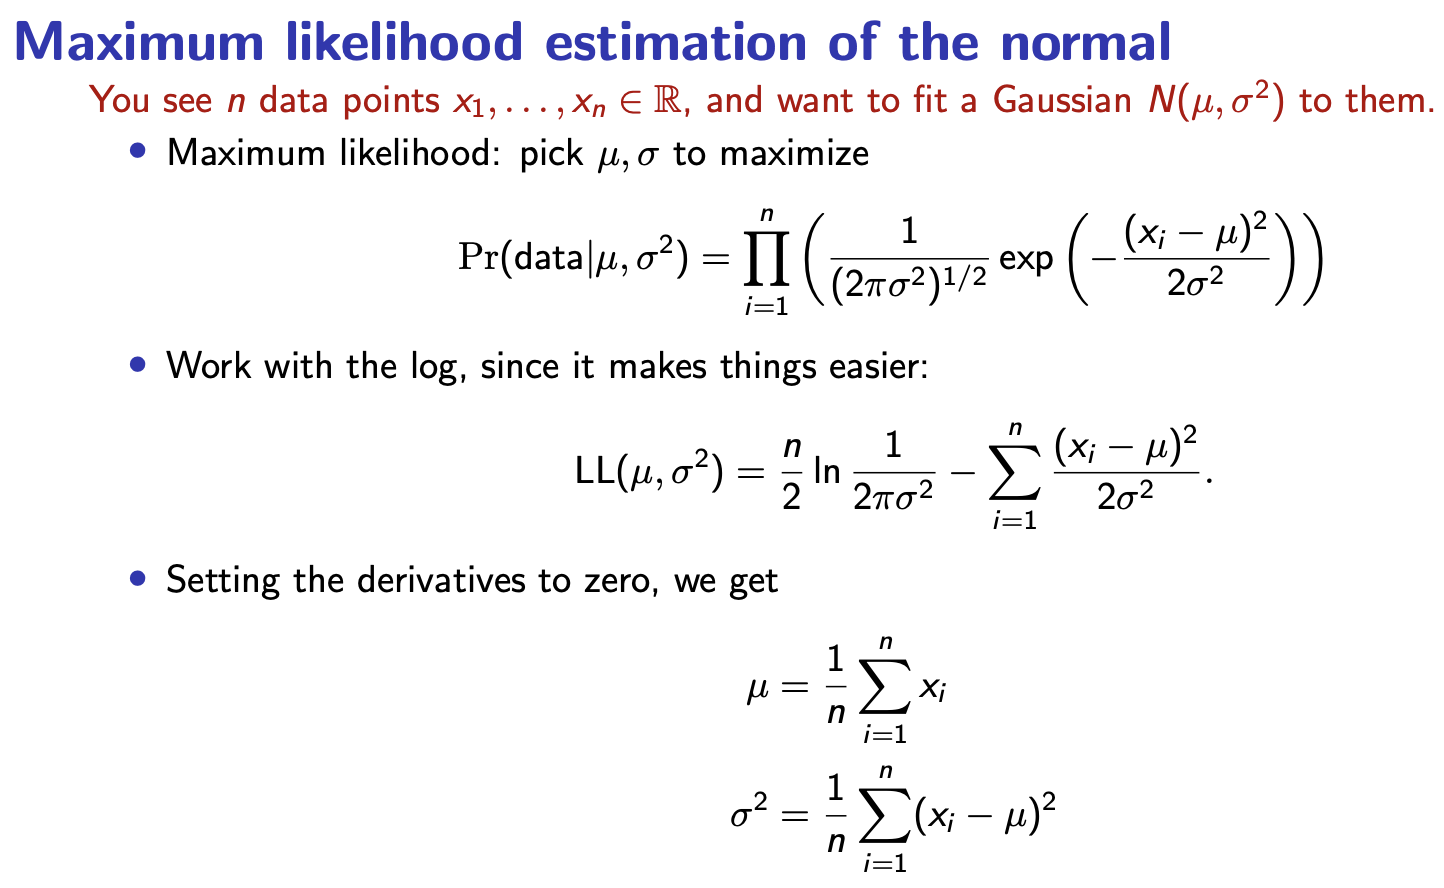
\includegraphics[scale=0.5]{normal_mle}
        
    \part Binomial Distribution: For $X \sim bin(n,p)$:
        \begin{itemize}
            \item $E(X) = np$
            \item $\operatorname{Var}(X) = np(1 - p)$
            \item $Pr(X = k) = \binom{n}{k}p^k(1 - p)^{n - k}$
        \end{itemize}
        
    \part Laplace Smoothing: when you toss a coin $n$ times and observe $k$ heads,
        estimate the bias as $p = \frac{k+  1}{n + 2}$
        
    \part RV normalization: normalize a random variable $X$ such that
        $$\frac{X - E(X)}{std(X)} \xrightarrow{d} N(0, 1)$$
        
    \part Multi-nominal Distribution: Imagine a $k$-faced die, with probabilities
        $p_1, ..., p_k$. We then have: \begin{itemize}
            \item $p_1 + ... + p_k = 1$
            \item $E(X) = (np_1, ..., np_k)$
            \item $Pr(n_1, ..., n_k) = \frac{n!}{n_1!...n_k!} p_1^{n_1} ...
                p_k^{n_k}$,
                
                and this is the way to place balls numbered 1 through $n$ into 
                bins numbered 1 through $k$:
                $$\binom{n}{n_1, ..., n_k} = \frac{n!}{n_1!...n_k!} p_1^{n_1}
                ... p_k^{n_k}$$
        \end{itemize}
\end{parts}

\question dependence-handout

\begin{parts}
    \part Correlation: \begin{itemize}
        \item Positively correlated: $E(XY) > E(X)E(Y)$
        \item Negatively correlated: $E(XY) < E(X)E(Y)$
        \item Not correlated: $E(XY) = E(X)E(Y)$
    \end{itemize}
    
    \part Covariance:
        \begin{align*}
            cov(X, Y) &= E((X - E(X))(Y - E(Y))) \\
                        &= E(XY) - E(X)E(Y)
        \end{align*}
    \part Correlation:
        $$corr(X, Y) = \frac{cov(X, Y)}{std(X)std(Y)}$$
        
    \part Bivariate Gaussian (Normal) Distribution
    
        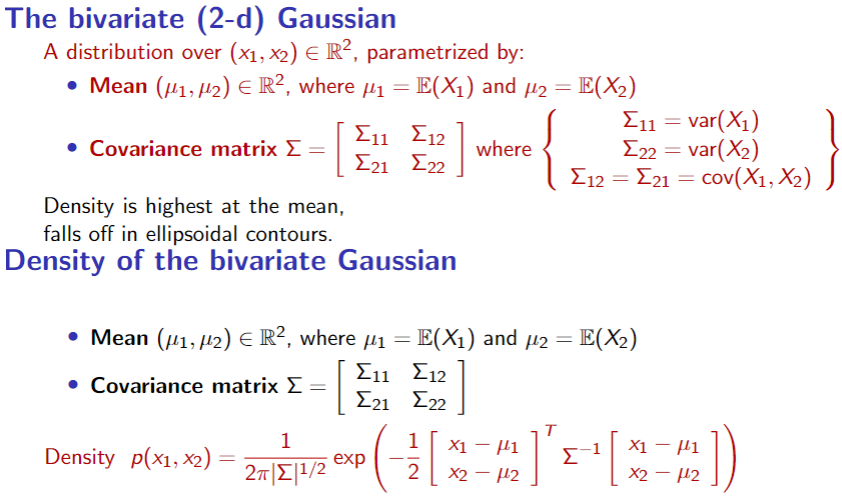
\includegraphics[scale=0.5]{biv_norm_props.png}
    
    \part Multivariate Gaussian (Normal) Distribution
    
        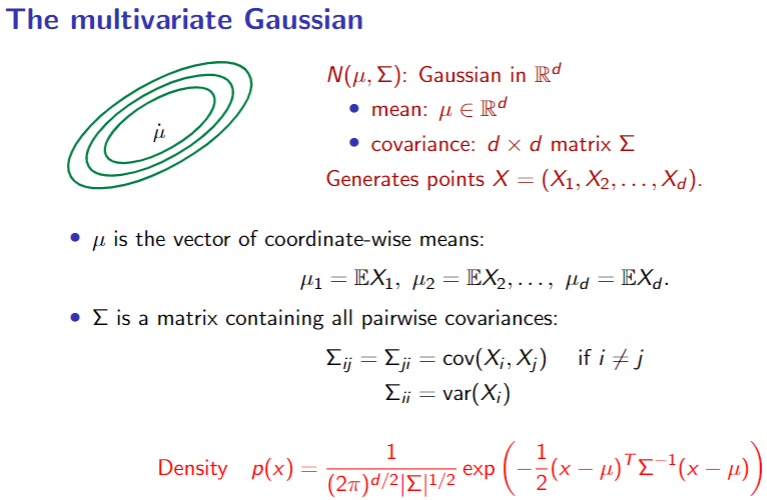
\includegraphics[scale=0.5]{multi_var_gaus_props.png}
        
    \part Diagonal Gaussian: when the $X_i$s are independent and 
        $\operatorname{Var}(X_i) = \sigma_i^2$, the covariance
        matrix is just:
        $$\Sigma = diag(\sigma_1^2, ..., \sigma_d^2)$$ with
        off-diagonal elements being all zeros.
        
        Each $X_i$ is an independent one-dimensional Gaussian
        $N(\mu_i, \sigma_i^2)$ such that:
        
        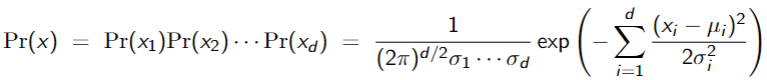
\includegraphics[scale=0.75]{diag_gaus_pr.png}
        
    \part Fit a Gaussian to data points $x^{(1)}, ..., x^{(m)} \in \bR^d$:
    \begin{itemize}
        \item Empirical mean $\mu = \frac{x^{(1)} + ... + x^{(m)}}{m}$
        \item Empirical covariance matrix has $i, j$ entry:
            $$\Sigma_{ij} = (\frac{1}{m}\Sigma_{k=1}^m x_i^{(k)}x_j^{(k)}) -
            \mu_i \mu_j$$
    \end{itemize}
    
\end{parts}

\question correlation-dependence-handout

\begin{parts}
    \part $X, Y$ are independent $\implies Cov(X, Y) = 0, Corr(X, Y) = 0$
    \part $Corr(X, Y) \neq 0 \implies X, Y$ are dependent 
    \part Correlation is the quick and dirty way to detect strong  dependencies,
        but it cannot find them all. 
    \part Correlation is not directional, and neither is covariance.
\end{parts}

\question \textbf{Side Notes}

Unrelated but useful: Quicksort \begin{itemize}
    \item Given an array $S[1 \dots n]$
    \item Split $S$ into 3 pieces: \begin{center}
        \item $S_L$ elements less than $v$
        \item $S_v$ elements equal to $v$
        \item $S_R$ elements larger than $v$
    \end{center}
    \item \textbf{Return} quicksort($S_L$) $\circ S_v \circ$ quicksort($S_R$)
\end{itemize}

\end{questions}

\end{document}